\newpage
\section{Anexo: Diagrama P \& ID} \label{anexopid}
	
	
\begin{figure}[h!]
	\centering
	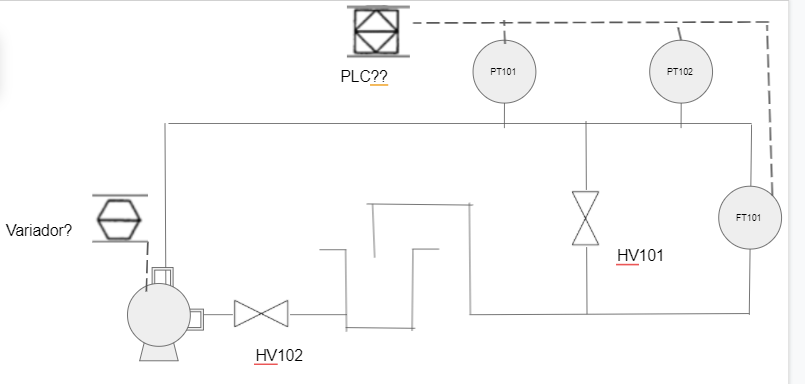
\includegraphics[scale=0.9 ,angle =90]{diag.png}
	\captionof{figure}{Diagrama p\&id}
\end{figure}

\newpage
\section{Anexo: Tabla de Direcciones ModBus} \label{Anexo1}


\begin{longtable}{|p{1.2cm} |p{4cm} |p{4cm} |p{1.5cm} |p{3.2cm} |}
	\caption{Tabla de variables y direcciones}
	\label{tab:direc}  \\
	
	\hline
	\multicolumn{1}{|c|}{\textbf{\begin{tabular}[c]{@{}c@{}}Tipo de \\ variable\end{tabular}}} & \multicolumn{1}{c|}{\textbf{TAG}} & \multicolumn{1}{c|}{\textbf{Descripción}} & \multicolumn{1}{c|}{\textbf{\begin{tabular}[c]{@{}c@{}}Tipo de \\ dato\end{tabular}}} & \multicolumn{1}{c|}{\textbf{Dirección}} \\ \hline
	\endfirsthead
	
	\multicolumn{5}{c}%
	{{\bfseries \tablename\ \thetable{} -- continuación}} \\
	\hline
	\multicolumn{1}{|c|}{\textbf{\begin{tabular}[c]{@{}c@{}}Tipo de \\ variable\end{tabular}}} & \multicolumn{1}{c|}{\textbf{TAG}} & \multicolumn{1}{c|}{\textbf{Descripción}} & \multicolumn{1}{c|}{\textbf{\begin{tabular}[c]{@{}c@{}}Tipo de \\ dato\end{tabular}}} & \multicolumn{1}{c|}{\textbf{Dirección}} \\ \hline
	\endhead
	
	\hline \multicolumn{5}{|r|}{{Sigue en la página siguiente}} \\ \hline
	\endfoot
	
	%\hline \hline
	\endlastfoot
	

	DO & PID\_XSMA0 & Habilitar control automatico manual & Boolean & Device0:000003 \\ \hline
	DO & VSD\_XSM0 & Marcha desde el hdmi & Boolean & Device0:000004 \\ \hline
	DO & VSD\_XST0 & Parada desde SCADA & Boolean & Device0:000005 \\ \hline
	DO & PLC\_XSDES & Desenclave de bomba & Boolean & Device0:000006 \\ \hline
	DO & PID\_XSA0 & PID modo automatico & Boolean & Device0:000008 \\ \hline
	DO & PID\_XSM0 & PID modo manual & Boolean & Device0:000009 \\ \hline
	DO & VSD\_XSFO & Restablecer fallas VSD & Boolean & Device0:000010 \\ \hline
	DI & VSD\_YHS0 & Parada de emergencia fisico & Boolean & Device0:000011 \\ \hline
	DI & VSD\_YLR0 & Modo fisico o scada & Boolean & Device0:000012 \\ \hline
	DI & PID\_YMA0 & Estado manual automatico & Boolean & Device0:000013 \\ \hline
	DI & PID0PIT1\_XRST & Restablecer valores PID & Boolean & Device0:000014 \\ \hline
	DI & PID0PIT2\_XRST & Restablecer valores PID & Boolean & Device0:000015 \\ \hline
	DI & PID0FT1\_XRST & Restablecer valores PID& Boolean & Device0:000016 \\ \hline
	AI & FT01 & Caudal & Float & Device0:400001 \\ \hline
	AI & VSD\_AI1C & Valor del pote & Float & Device0:400003 \\ \hline
	AI & VSD\_IC000 & Corriente & Float & Device0:400005 \\ \hline
	AI & VSD\_SC000 & Frecuencia & Float & Device0:400007 \\ \hline
	AI & VSD\_JC000 & Potencia & UInt & Device0:400009 \\ \hline
	AI & VSD\_WC000 & Torque & UInt & Device0:400011 \\ \hline
	AI & VSD\_EC000 & Voltaje & Float & Device0:400013 \\ \hline
	AI & PIT02 & Presion2 & Float & Device0:400015 \\ \hline
	AI & PIT01 & Presion1 & Float & Device0:400017 \\ \hline
	AI & VSD\_SC001 & Velocidad & UInt & Device0:400019 \\ \hline
	AI & TE001 & Temperatura & Float & Device0:400021 \\ \hline
	AI & PID\_SY000 & Accion de control & Float & Device0:400023 \\ \hline
	AI & VSD\_R\_ERR & Errores, tabla de errores & UInt & Device0:400025 \\ \hline
	AI & PID0PIT1\_TD\_LAG & P1 TD LAG & Float & Device0:400047 \\ \hline
	AI & PID0PIT2\_TD\_LAG & P2 TD LAG & Float & Device0:400049 \\ \hline
	AI & PID0FT1\_TD\_LAG & F1 TD LAG & Float & Device0:400051 \\ \hline
	AI & PID\_SR00 & Valor manual, control desac & Float & Device0:400053 \\ \hline
	AI & PID0PIT1\_SP & Valor Ref P1 & Float & Device0:400057 \\ \hline
	AI & PID0PIT2\_SP & Valor Ref P2 & Float & Device0:400059 \\ \hline
	AI & PID0FT1\_SP & Valor Ref F1 & Float & Device0:400061 \\ \hline
	AI & PID0PIT1\_KI & P1 KI & Float & Device0:400063 \\ \hline
	AI & PID0PIT1\_KP & P1 KP & Float & Device0:400065 \\ \hline
	AI & PID0PIT1\_KD & P1 KD & Float & Device0:400067 \\ \hline
	AI & PID0PIT2\_KI & P2 KI & Float & Device0:400071 \\ \hline
	AI & PID0PIT2\_KP & P2 KP & Float & Device0:400073 \\ \hline
	AI & PID0PIT2\_KD & P2 KD & Float & Device0:400075 \\ \hline
	AI & PID0FT1\_KI & F1 KI & Float & Device0:400077 \\ \hline
	AI & PID0FT1\_KP & F1 KP & Float & Device0:400079 \\ \hline
	AI & PID0FT1\_KD & F1 KD & Float & Device0:400081 \\ \hline
	AI & PID\_SEL & Seleccionar control P1 P2 F1 & UInt & Device0:400083 \\ \hline
	DR & VSD\_ETI & Motor encendido o apagado & Boolean & Device0:400101:4 \\ \hline
	DR & YS\_AP & Alta presion & Boolean & Device0:400103:0 \\ \hline
	DR & YS\_SC & Sin Caudal & Boolean & Device0:400103:1 \\ \hline
	DR & YS\_SP1 & Sin Sensor P1 & Boolean & Device0:400103:2 \\ \hline
	DR & YS\_SP2 & Sin Sensor P2 & Boolean & Device0:400103:3 \\ \hline
	DR & YS\_AT & Alta Temp & Boolean & Device0:400103:4 \\ \hline
	DR & FT01\_YCOM & Sin Caudal & Boolean & Device0:400103:5 \\ \hline
	DR & VSD\_YCOM & Sin comu con variador & Boolean & Device0:400103:6 \\ \hline
	%	\\*
	%	\caption{Tabla de variables y direcciones}
	%	\label{tab:direc}  	
	
	
\end{longtable}

\newpage

\section{Anexo: Manual BANCO-SCADA}
\subsection{Características generales}
\begin{itemize}
	\item Utilizado en sistema operativo Windows 10 o mayor.
	\item Posibilidad de utilizar el banco de pruebas de modo remoto o local.
	\item Generado para controlar tres variables distintas, dos de presión o caudal.
\item Posibilidad de generar perturbaciones en el sistema para observar distintas respuestas.
	\item Fácil de transportar.
\item Posibilidad de guardar valores como históricos y ver datos en tiempo real.
\end{itemize}


\subsection{Guía de uso}
\begin{enumerate}
	\item Conectar el banco de pruebas con los respectivos sensores y transductores en el módulo correspondiente del PLC.
	\item Conectar cable Ethernet en el PLC a un router o PC.
	\item Alimentar el sistema con alimentación trifásica y 220V.
	\item Abrir iFix y la tabla de variables y el archivo con extensión .mbe dónde se procederá a conectar el sistema SCADA a la misma red en la que se encuentra el PLC.
	\item Comprobar comunicación al correr SCADA.
\end{enumerate}

\subsubsection{Pantalla PRINCIPAL}

\begin{figure}[h!]
	\centering
	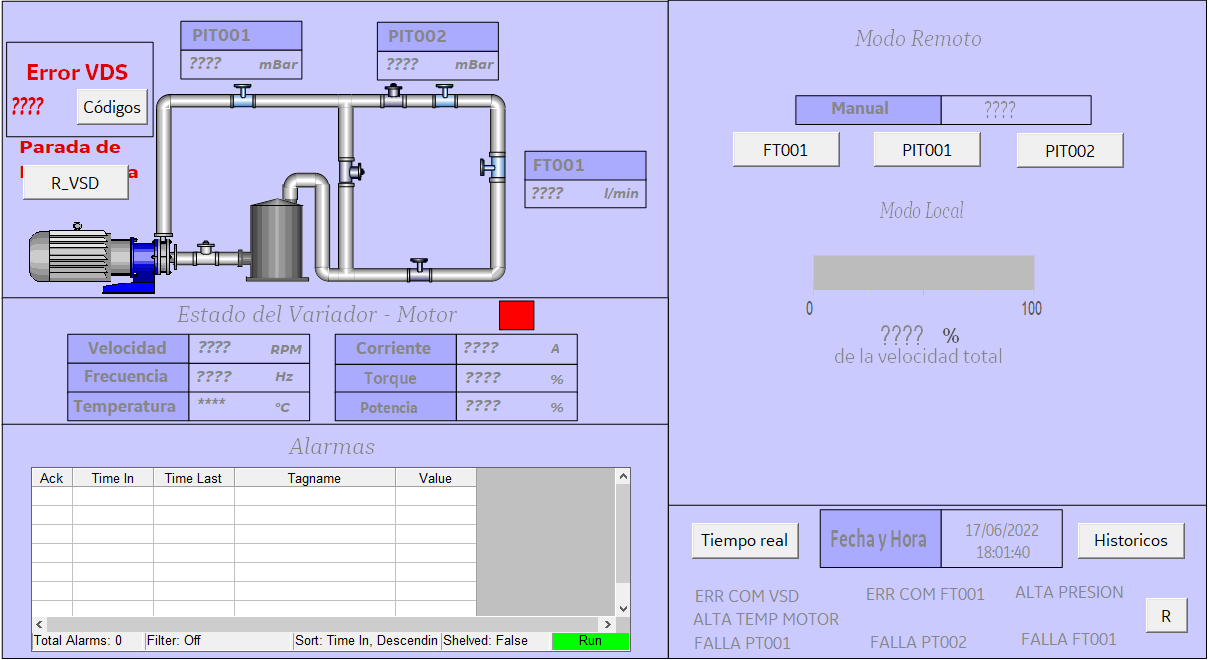
\includegraphics[width=0.9\linewidth]{pantalla1.png}
	\captionof{figure}{Pantalla principal}
	\label{fig:pantalla1}
\end{figure}
\begin{figure}[h!]
	\centering
	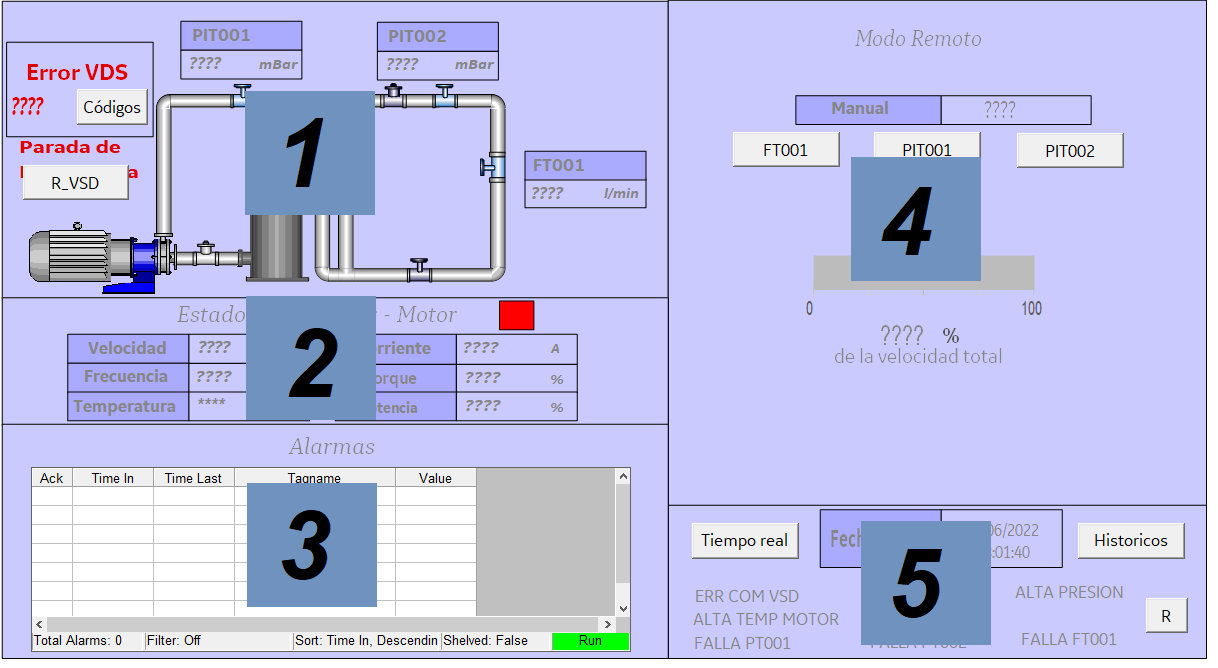
\includegraphics[width=0.6\linewidth]{p_partes.png}
	\captionof{figure}{Partes del sistema SCADA}
	\label{fig:partes}
\end{figure}

\paragraph{Diagrama del banco de pruebas}
Se observan los valores de presión y caudal en un diagrama similar al banco de prueba físico. A la izquierda se mostrará el último error el cúal puede observarse en la tabla que se abre al hacer click en el botón A. Si se desea restaurar el valor se debe presionar el botón B (Figura \ref{fig:pp1}).
\begin{figure}[h!]
	\centering
	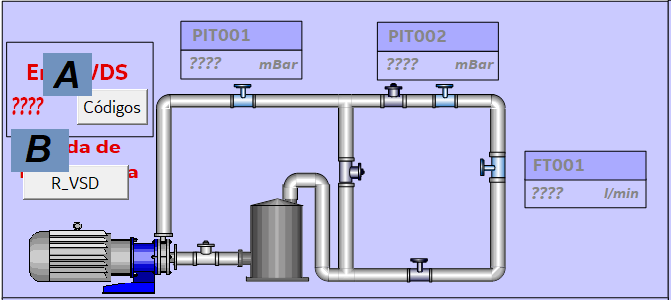
\includegraphics[width=0.6\linewidth]{p_p1.png}
	\captionof{figure}{Subpantalla 1}
	\label{fig:pp1}
\end{figure}

\paragraph{Estado del variador - Motor}
En esta sección se ve de forma lumínica en color rojo si el motor está prendido indica señal de cuidado o alerta; mientras que en color verde que el motor está apagado. Se observan variables de velocidad del motor, frecuencia del motor, temperatura obtenida por el termistor, corriente, torque y potencia consumida por el motor.
\paragraph{Alarmas}
Sección destinada al alarmero dónde muestra el período de tiempo que ocurrió el hecho, el nombre de la variable y el valor alcanzado.
\paragraph{Modo remoto/ Modo local}
\begin{itemize}
	\item Modo Local\\
	Si la llave selectora del banco de pruebas se encuentra seleccionado el modo local, se observará el cartel en esta sección centrado que expresará que se encuentra en modo local (Figura \ref{fig:localremoto}.a).
	\item Modo Remoto\\
	Si la llave selectora del banco de pruebas se encuentra seleccionado el modo remoto, el sistema está preparado para recibir órdenes desde el sistema SCADA. El motor puede encenderse con velocidad 0 al presionar la tecla A o encender a una velocidad preestablecida colocando previamente un valor entero en RPM entre 0 y 3600 y luego presionar la tecla A (Figura \ref{fig:localremoto}.b). 
	
	Si se desea se puede abrir cada ventana del lazo de control (Figura \ref{fig:LC}) botones B dónde muestra el valor de cada variable PID, pudiéndose colocar otros valores mientras que se use la coma como separador decimal. Con el botón C, se podrá restablecer los valores del PID cuyos valores fueron fijados al momento de realizar el proyecto, dónde las respuestas se muestran en las figuras PONER TIPO LA COMPARACION DE PID PERO CON SOLO EL QUE SE UTILIZA Y Q SE LEEAN LOS VALORES DE PID. 
	
	Al presionar el botón automático (D), se cierra el lazo del sistema y puede establecerse la presión o caudal deseado en E, dónde la coma será el separador decimal y los rangos serán según tabla \ref{tab:rang}. En caso de presionar y que quede manual (D) los valores se establecerán según \textit{Manual} (Figura \ref{fig:localremoto}.b). 
\end{itemize}

\begin{figure}[htbp]
	\centering
	\subfigure[Modo local]{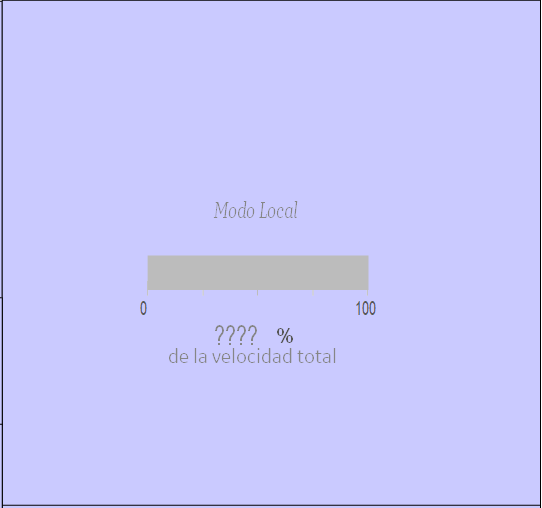
\includegraphics[width=60mm]{p_4c.png}}
	\subfigure[Modo remoto]{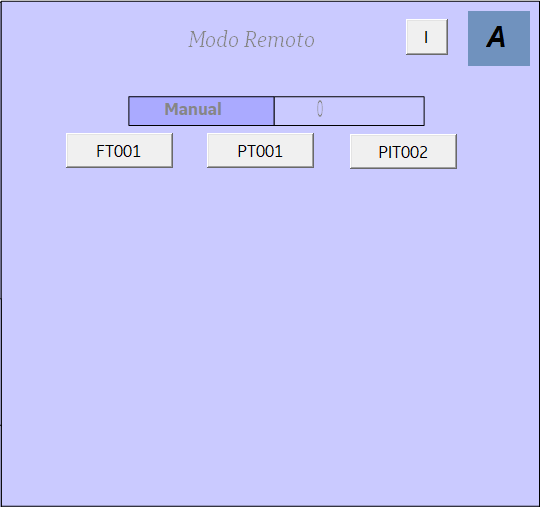
\includegraphics[width=60mm]{p_4b.png}}
	\caption{Subpantalla 4} \label{fig:localremoto}
\end{figure}

\begin{figure}[h!]
	\centering
	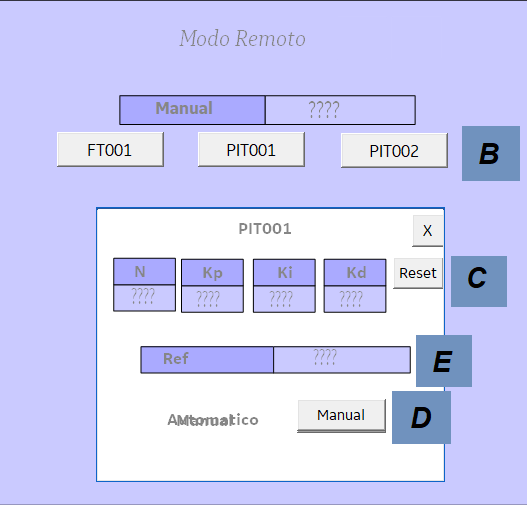
\includegraphics[width=60mm]{p_4a.png}
	\captionof{figure}{Modo lazo cerrado}
	\label{fig:LC}
\end{figure}
\begin{table}[]
	\centering
	
	\begin{tabular}{|cc|l|c|}
		\hline
		\multicolumn{2}{|l|}{\textbf{Variable}} & \textbf{Rango} & \multicolumn{1}{l|}{\textbf{Unidades}} \\ \hline
		\multicolumn{1}{|c|}{\textbf{PIT001}} & Presión & 60 - 930 & mbar \\ \hline
		\multicolumn{1}{|c|}{\textbf{PIT002}} & Presión & 60 - 700 & mbar \\ \hline
		\multicolumn{1}{|c|}{\textbf{FT001}} & Caudal & 2 - 11,7 & l/min \\ \hline
	\end{tabular}
\caption{Rangos de las variables}
\label{tab:rang}
\end{table}

\paragraph{Fallas y ventanas de gráficos}
En la pantalla 5 se observan los carteles de eventuales fallas que puedan ocurrir en el sistema, pudiéndolo reanudar con el botón que tiene la letra R.

Otra de las cosas que tiene esta subpantalla es la fecha y hora y dos botones dónde al presionarlos se abren pantallas para observar gráficamente datos en tiempo real o de forma histórica.

\subsubsection{Pantalla datos en tiempo real}
En la figura \ref{fig:scadaTR} se puede observar la pantalla de los datos en tiempo real (la imagen no corresponde a valores reales tomados durante las pruebas).
\begin{figure}[h!]
	\centering
	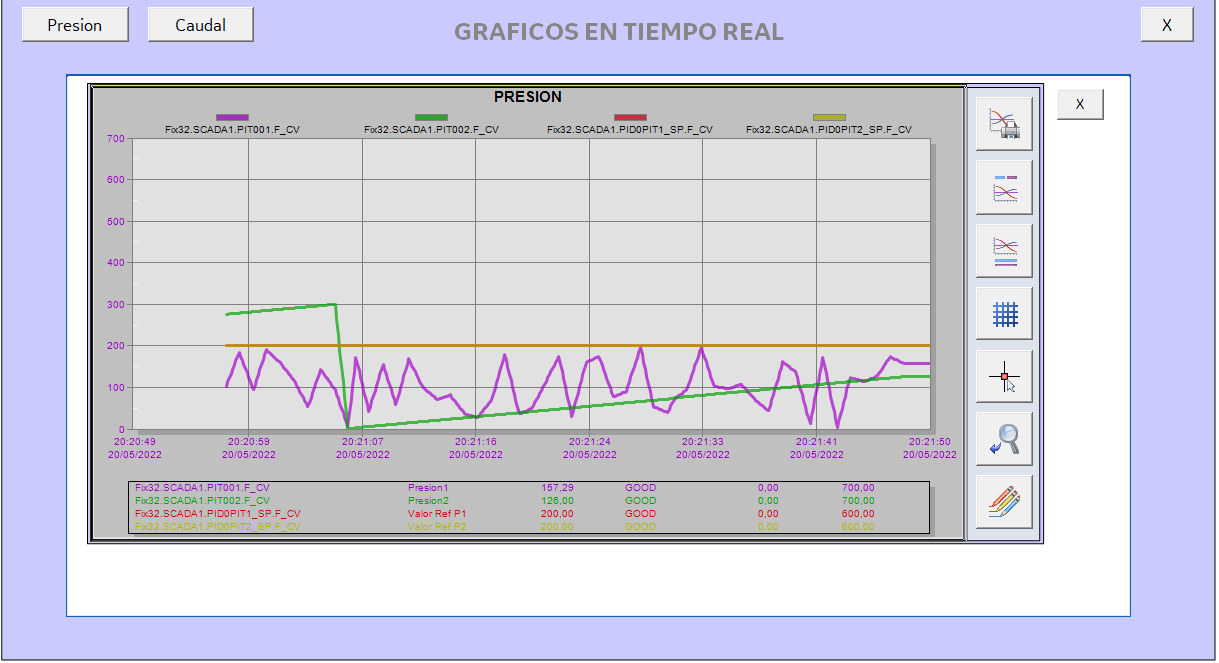
\includegraphics[width=1\linewidth]{scadaTR.png}
	\captionof{figure}{Pantalla datos en tiempo real}
	\label{fig:scadaTR}
\end{figure}

\subsubsection{Pantalla datos histórico}

Para interpretar datos históricos se puede por dos métodos, uno es generar un archivo .txt y el otro es de forma gráfica. 
Se generó una pantalla SCADA prediseñada de \textit{iFix} dónde al conectar con el servidor \textit{Historian}, busca los datos históricos de la variable elegida y guarda un archivo \textit{.txt} con el horario y valores. Se puede elegir más de una variable, pero se debe tener en cuenta que no se generan columnas nuevas sino que generará en el mismo archivos más filas (Figura \ref{fig:grafhist} a).\\
Otra de las opciones es observar datos históricos en un gráfico de tiempo, estas variables están preestablecidas y son las presiones y el caudal con sus respectivos valores de referencias (Figura \ref{fig:grafhist} b).


\begin{figure}[htbp]
	\centering
	\subfigure[Gráficos de datos históricos]{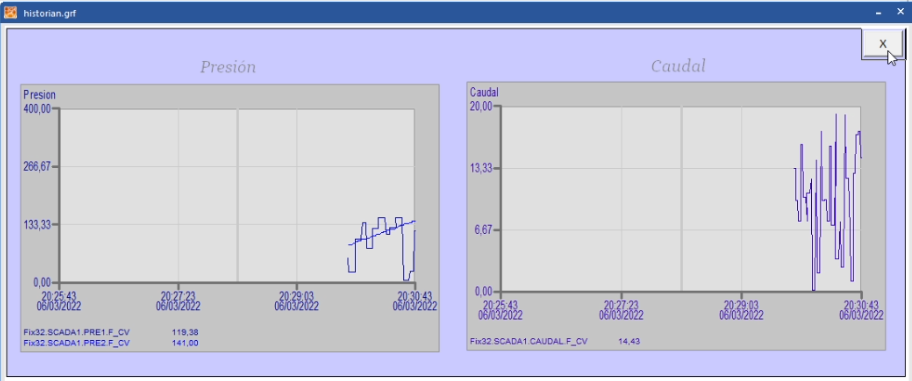
\includegraphics[width=1\linewidth]{scada3.png}}
	\subfigure[Guardado de datos históricos]{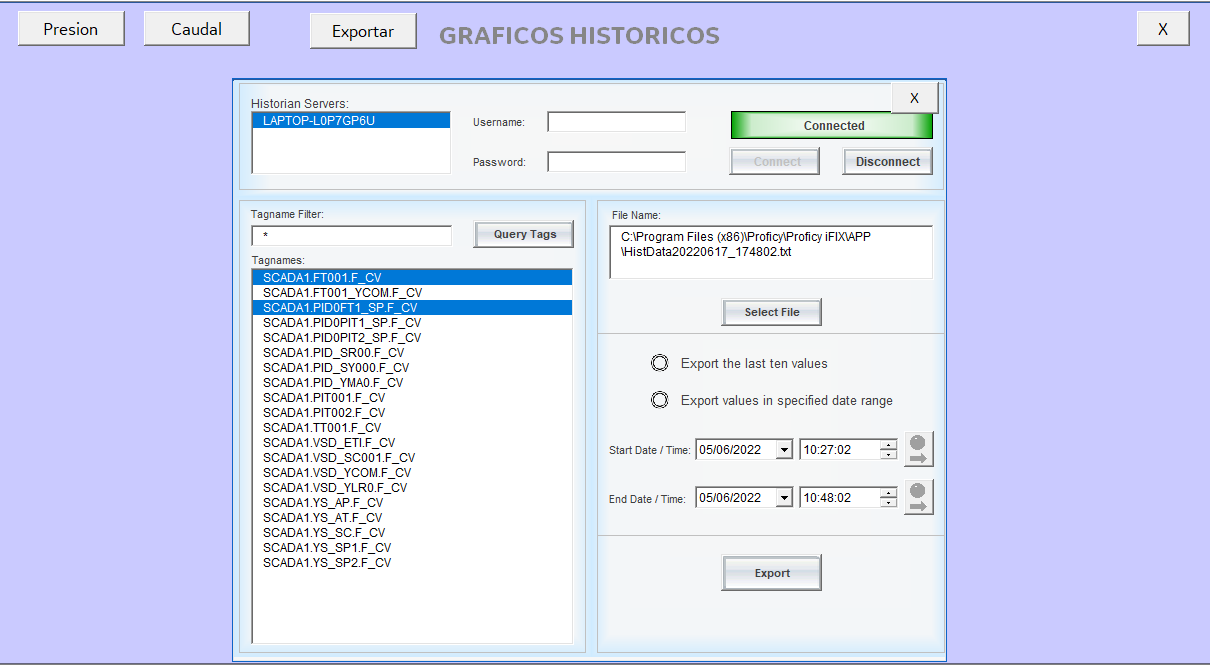
\includegraphics[width=1\linewidth]{scada33.png}}
	\caption{Datos históricos} \label{fig:grafhist}
\end{figure}





\newpage